\documentclass[10pt]{article}
\newcommand\mycommfont[1]{\small\ttfamily\textcolor{red}{#1}}
\usepackage{amsmath,amsthm,mathtools,commath,xcolor,graphicx,algorithmic,algorithm}
\graphicspath{ {./} }
\title{TDA251\\Solutions for Assignment 3}
\author{Wang QuFei\\900212-6952\\qufei@student.chalmers.se}

\begin{document}
\maketitle
\section*{Excrcise 5}
\textbf{5.1} A deterministic algorithm can be given as follows:
\begin{enumerate}
	\item Denote $c$ as the latest known contaminated node, initialize $c$ with root.
	\item Check whether the left child of $c$ is contaminated, if it is true, then assign this node as the new value of $c$, and repeat this step.
	\item Check whether the right child of $c$ is contaminated, if it is true, then assign this node as the new value of $c$, and go back to step 2.
	\item Return the current value of $c$ as the node $p$ being searched.
\end{enumerate}
It can be seen from this process that, in the worst case, $2k + 2$ tests are needed, which is bound in $2k + O(1)$.\\
\textbf{5.2} A randomized algorithm can be given as follows:
\begin{enumerate}
	\item Denote $c$ as the latest known contaminated node, initialize $c$ with root.
	\item Randomly test one of the children of $c$ with probability $1/2$, if the tested node is contaminated, assign it as the new value of $c$, and repeat this step.
	\item Test the other child of $c$, if it is contaminated, assign it as the new value of $c$, and go back to step 2.
	\item Return the current value of $c$ as the node $p$ being searched.
\end{enumerate}
Let $X$ be the random variable representing the number of tests needed to find the $k$ contaminated edges. Denote $X_{i}$ as the random variable representing the number of tests needed to find the $ith$ contaminated edge. Then we have
	\[X = \sum_{i}X_{i}\]
The expected value of $X_i$ is
	\[E[X_i] = 1 \times \frac{1}{2} + 2 \times \frac{1}{2} = 1.5\]
By linearity of expectation, the expected value of $X$ is
	\[E[X] = \sum_{i}E[X_i] = 1.5k\]
After the $kth$ contaminated edge is found, two more checks are needed to make sure there's no further contamination, so the expected number of this randomized algorithm is $1.5k + O(1)$.\\
\textbf{5.3} A randomized algorithm with further improved expected testing numbers is given as follows. The basic idea is to find the contaminated nodes for every two consecutive contaminated edges.\\
\begin{figure}[h]
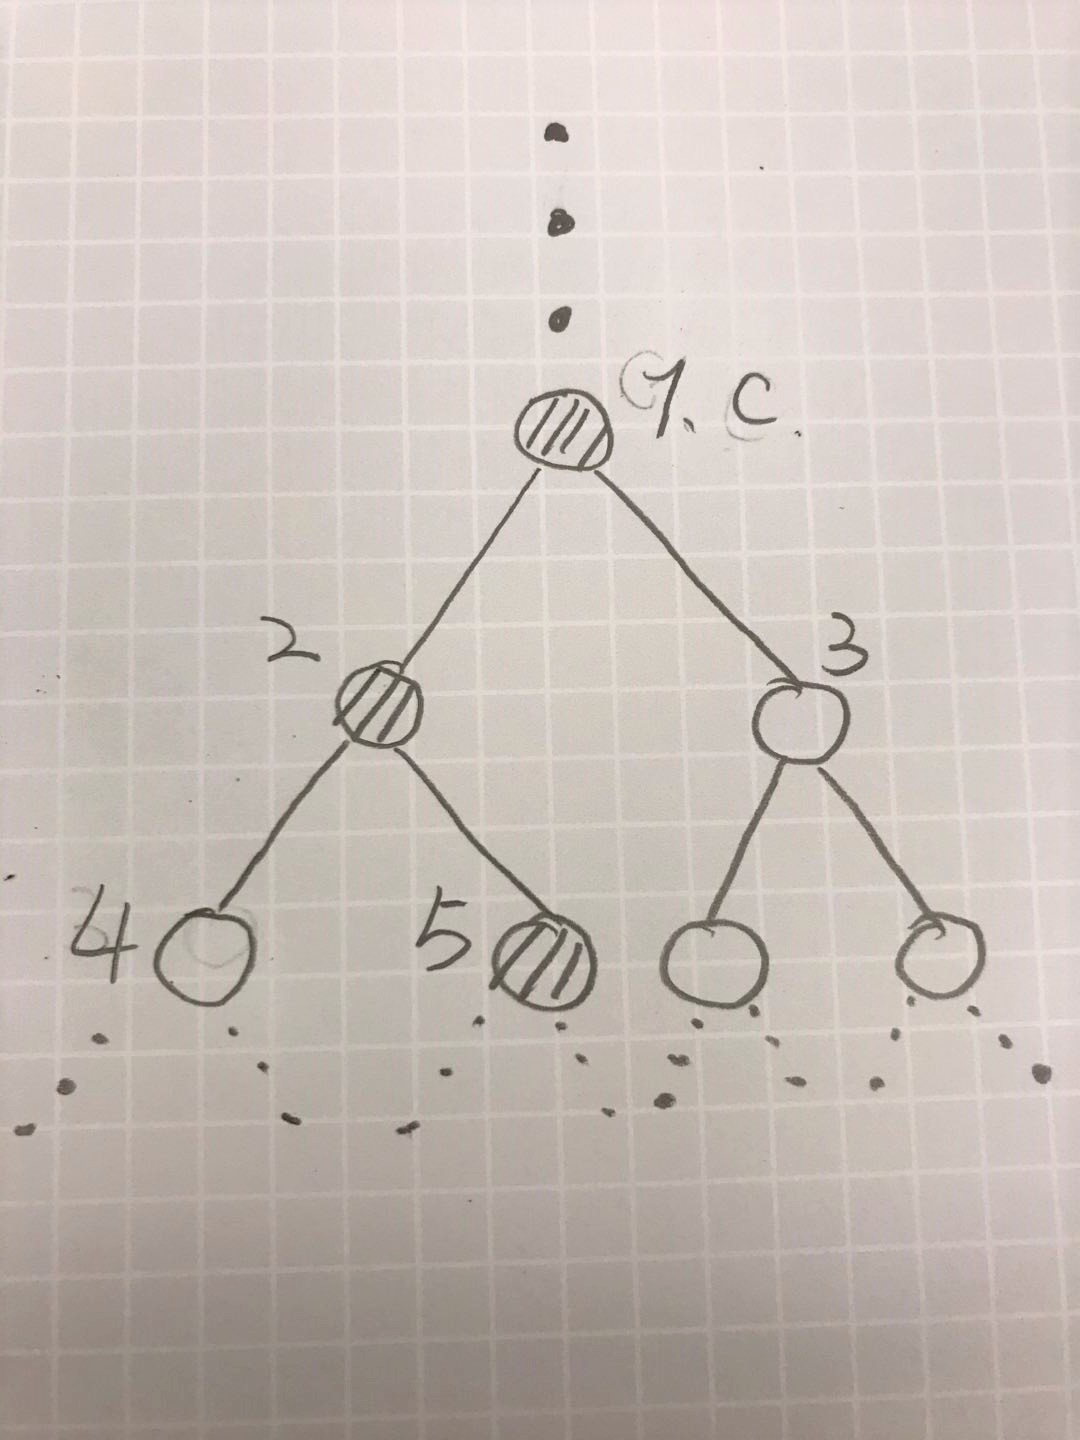
\includegraphics[width=6cm, height=7cm]{1}
\centering
\end{figure}
As the image here shows, suppose we have node $1$ confirmed as the latest contaminated node, it is denoted as $c$ and the partial polution path is $(1 \to 2 \to 5)$. Now the algorithm proceeds as follows:
\begin{enumerate}
	\item Randomly check $2$ or $3$ with probability $1/2$
	\item If $2$ is choosen for the check, then we could know that it is polluted. Further, we check $4$ or $5$ randomly with probability $1/2$. If $5$ is choosen, then we confirm  2,5 as polluted nodes in 2 checks, with probability $1/4$; Otherwise, if $4$ is choosen, then by one more check, we can confirm nodes $2,5$ as polluted nodes in 3 checks, with probability $1/4$.
	\item If 3 is choosen in step 2, we could know it is not polluted.  Further, we check $4$ or $5$ randomly with probability $1/2$. If $5$ is choosen, then we confirm 2,5 as polluted nodes in 2 checks, with probability $1/4$; Otherwise, if $4$ is choosen, then by one more check, we can confirm  2,5 as polluted nodes in 3 checks, with probability $1/4$.
	\item Mark node 5 as the new value of $c$, and repeat this procedure until the final stage.
	\item In the final stage, we either have one more contaminated node to find, or all contaminated nodes have already been found, we just don't know it because $k$ is unknown. In either case, at most a constant number of extra checks are needed to reach to a conclusion. For example, suppose the current value of $c$ is the last node(using the same image), then we have checks either $[2,4,5,3]$ or $[3,5,4,3]$ or $[3,4,5,2]$ or [3,5,4,2] needed to reach to a conclusion. The analysis of the case when $2$ or $3$ is the last node with 1 being established as the latest confirmed contaminated node is similar.
\end{enumerate}
In stages where two consecutive contaminated edges exist, the expected number of checks is 
\[(\frac{1}{4} \times 2 + \frac{1}{4} \times 3) \times 2 = \frac{5}{2}\]
The number of such stages is of size $O(k/2)$, so the total number of expected checks is
\[\dfrac{5}{4}k + O(1)\]
\qed
\section*{Excrcise 6}
{\color{red}
An obvious lower bound on the value  $\sum_{i=1}^{m}(r_{\pi}(S_i) - l_{\pi}(S_i))$ is $\sum_{i=1}^{m}(|S_i| - 1)$. It can be obtained by having a permutation which enables all the elements from each $S_i$ being placed compactly on a continuous sequence of shelves. \\
Suppose $V = \{a, b, c, d\}$ and $S_1 = \{a, c, d\}$, permutations in forms such as $[b, c, d, a]$, $[d, a, c, b]$ enable items from $S_1$ being placed compactly, whereas permutations such as $[a, c, b, d]$ or $[c, d, b, a]$ don't, because an extra element `b' is placed among them. The effect of such `non-compact' permutation is to increase the value $r_{\pi}(S_i) - l_{\pi}(S_i)$ for a particular $S_i$ by the number of extra elements placed among its items, from the optimal value $|S_i| - 1$. In the example above, both $[a, c, b, d]$ and $[c, d, b, a]$ cause the value $r_{\pi}(S_1) - l_{\pi}(S_1)$ from the optimal 2 to 3.\\
In the following context, for each given $S_i$, we call a position in a permutation as `extra', when
\begin{enumerate}
\item The element placed on this position does not belong to $S_i$.
\item The positions before it contain an(some) element(s) from $S_i$, but not all of them.
\end{enumerate}
Our definition of `extra position' relates to the order of items in the sense that, still taking $V$ and $S_1$ mentioned above as an example, suppose other elements are added to $V$, for permutations start with $[a, b, \dots]$, then the existence of `b' in the second position(which is deemed as `extra') will contribute 1 to the value $r_{\pi}(S_1) - l_{\pi}(S_1)$ from its optimal lower bound $|S_1| - 1$, no matter how the rest of the elements from $V$ are arranged. This is a cost which will not be caused by a permutation starts with $[b, a, \dots]$, where the replacement of element `b' from 2 to 1 preserves the possibility that all items from $S_1$ still placed compactly.}\\
Our goal is to keep the total number of such extra postions as small as possible, so that the real target value $\sum_{i=1}^{m}(r_{\pi}(S_i) - l_{\pi}(S_i))$ is minimized.\\
Define $obj(k, W)$ as the minimum of the sum of the extra positions, given that the first $k$ shelves are occupied by items from $W \subseteq V$. Let $obj(0, W) = 0$, $obj(k, \emptyset) = 0, k > 0$, the formula to calculate $obj(k,W)$ can be given as:
	\[obj(k, W) = \min_{v \in W}\{\delta_{v,k} + obj(k-1, W \setminus \{v\})\}\]
$\delta_{v,k}$ is the number of the extra positions caused by placing $v$ on shelf $k$, given that the first $k-1$ shelves are occupied by items from $W \setminus \{v\}$. It is calculated by the following procedure:
\begin{algorithmic}
\STATE \textbf{Initialization:} $\delta_{v,k} = 0$, $A := W \setminus \{v\}$
\FOR{$i=0$ to $m$}
	\IF{$S_i \cap A \neq \emptyset$}
	\STATE $B := S_i \setminus A$
		\IF{$B \neq \emptyset$ \AND $v \notin B$}
		\STATE $\delta_{v,k} = \delta_{v,k} + 1$
		\ENDIF
	\ENDIF
\ENDFOR
\end{algorithmic}
This procedure is straightforward: For all $S_i$, if $S_i \cap A \neq \emptyset$ and there are still elements in $S_i$ not included, when $v \notin B$, then one extra position is counted.\\
The time bound of this algorithm is $O^{*}(2^n)$, since the size of the powerset of $V$ is $2^{n}$, the steps to calculate $obj(k, W)$ for a given $k$ bounds in $O(n)$, the time bound to calculate $\delta_{v,k}$ is $O(m)$.\\
The real target value can be calculated by 
	\[\sum_{i=1}^{m}(r_{\pi}(S_i) - l_{\pi}(S_i)) = obj(n, V) + \sum_{i=1}^{m}(|S_i| - 1)\]
An actual permutation which leads to the optimal value can be obtained by recording the partial result of $obj(k, W)$ along with its permutation through the procedure.\\
\qed
\end{document}